\documentclass{siamart1116}
\usepackage{amsmath, amssymb}
%\usepackage{amsmath,amssymb,amsfonts,graphicx,amsthm,dsfont}
%\usepackage{listings}
%\usepackage{courier}
\usepackage{enumerate}
%\usepackage{color}
%\usepackage[usenames,dvipsnames]{xcolor}
%\usepackage{hyperref,tikz,mdframed}
%\hypersetup{colorlinks=true,urlcolor=MidnightBlue,citecolor=PineGreen,linkcolor=BrickRed}

% \lstset{
% 	basicstyle=\small\ttfamily,
% 	keywordstyle=\color{blue},
% 	language=python,
% 	xleftmargin=16pt,
% }
\usepackage{algorithmicx}
\usepackage{algpseudocode}% http://ctan.org/pkg/algorithmicx
\usepackage{float}

\textwidth=5.8in
\textheight=9in
\topmargin=-0.5in
\headheight=0in
\headsep=.5in
\hoffset  -.4in
\pagestyle{empty}

\newcommand{\Fp}{\mathbb{F}_p}
\newcommand{\Q}{\mathbb{Q}}
\newcommand{\Z}{\mathbb{Z}}
\newcommand{\kron}[2]{\left(\frac{#1}{#2}\right)}
\newcommand{\Aut}{\mathrm{Aut}}
\newcommand{\End}{\mathrm{End}}
\newcommand{\SO}{\mathrm{SO}}
\newcommand{\SU}{\mathrm{SU}}
\newcommand{\tr}{\operatorname{tr}}
\newcommand{\dee}{\mathrm{d}}
\newcommand{\deee}{\textbf{\text{\emph{d}}}}

\newcommand{\md}[1]{\textcolor{cyan}{#1}}

\newcommand{\TheAuthors}{V. Chen\\ Advised by A. M. Stuart and  M. M. Dunlop}

%\newtheorem{theorem}{Theorem}
%\newtheorem{definition}{Definition}

\graphicspath{ {graphics/} }

\title{SURF 2017 Interim Report 1}
\author{\TheAuthors}
\date{}
\begin{document}
\maketitle
\setlength{\unitlength}{1in}
\setlength{\parindent}{0in}

\section{Introduction}
%%%%% will eventually need more background -- definition of graph laplacian, weights, use in unsupervised learning, fiedler vector, etc
In the context of semi-supervised learning, the \textit{clustering} problem refers to attempting to group a set of data or objects into clusters of similar objects. Applications of clustering include image segmentation, social network analysis, and voter classification, but the reader will readily identify numerous other potential applications. We approach the clustering problem from a graph-theoretical point of view, which assigns a node to each data value and weights on edges between nodes to indicate how related the data points are.

Let $Z$ be a set of nodes $\{1, \ldots N\}$. The feature vectors are given by $x : Z \rightarrow \mathbb{R}^d$. $Z' \subset Z$ is a subset of labeled nodes, for which we have label data given by $y : Z' \to \{-1, 1\}$ for {\bf binary} data, and $y : Z' \to \{e^1, \ldots e^k\}$ for {\bf $k$-ary} (multiclass) data.


The classifying function is given by the vector $u$, and the label model is given by $y(\ell) = S(u(\ell))$ for $l \in Z'$ (with possible additional corruption by noise). In the case of binary data, $y(\ell) \in \{\pm 1\}$, and for $v \in \mathbb{R}$,
\[
S(v) = \begin{cases}
1 & v>0\\
0 & v=0\\
-1 & v<0
\end{cases}
\]

In the case of multiclass data, $y(\ell) \in \{e^1, \ldots e^k\}$, $v \in \mathbb{R}^k$ and
\[
S(v) = e^p, \quad p = \underset{r =1,\ldots,k}{\mathrm{argmax}}\;v_r
\]
where $\{e^l\}_{l=1}^k$ denotes the standard basis of $\mathbb{R}^k$.

Given this problem, one goal is to come up with a classification that best fits the data. The research group in which I am working is currently looking at the effectiveness of incorporating Bayesian inference into semi-supervised learning. In the Bayesian approach, the unknown classifying function $u$ is viewed as a random variable, whose distribution is determined by combining the labeling model $y$ with a probability distribution representing our prior beliefs about the classification and derived from the feature vectors. Hierarchical Bayesian methods provide additional flexibility by introducing hyperparameters governing the prior distribution, which are in turn treated as random variables to be inferred.

Our prior beliefs come from \textit{spectral clustering}, which uses the clustering properties of the eigenvalues and eigenvectors of the graph Laplacian, a matrix defined on the similarity graph constructed from the feature vectors as follows:

Let the similarity graph be $G$ with weights $w_{ij} \ge 0$. A larger weight indicate a higher degree of similarity between the two nodes. Define $\delta_i = \sum_{k=1}^n w_{ij}$. Then, define matrices $W, D$ as:

\[W = w_{ij}, D = \begin{cases} 
\delta_i    & i = j \\
0           & i \neq j 
\end{cases}\]

Then, let $L = D - W$ denote the unnormalized graph Laplacian on $\mathbb{R}^N$. Denote the eigenbasis of $L$ by
\begin{equation}
\label{eqn:laplacian}
Lq_j = \lambda_j q_j,\quad j=0,\ldots,N-1.
\end{equation}

The graph Laplacian is important because the eigenvectors corresponding to the smaller eigenvalues are known to hold information about cluster data. In particular, if the graph has ``ideal'' clusters so that the edges between clusters all have weight 0, then the graph Laplacian would have as many eigenvalues 0 as there are clusters, and corresponding eigenvectors would be indicators for the clusters \cite{Spectral}. Even if the data is not ideal, the eigenvectors corresponding to small eigenvalues should hold clustering information. This includes the important Fiedler vector, the second-smallest eigenvector which is useful for bi-partitioning the graph. The eigenvalues and eigenvectors of the graph Laplacian are used to construct the prior probability distribution about $u$.

% Derivation of prior, likelihood

For the Bayesian approach, the prior, likelihood and posterior are defined as follows:
\begin{itemize}
\item[$\mathbb{P}(u)$:] Prior distributed as $N(0,C)$ where the covariance matrix $C = (L + \tau^2I)^{-\alpha}$. A sample $u$ from the prior can be made through a realization of the following random sum:
\begin{equation}
\label{eqn:prior}
u = \sum_{j=0}^M (\lambda_j + \tau^2)^{-\alpha/2}\xi_j q_j,\quad \xi_j\sim N(0,1) \quad \text{i.i.d.}
\end{equation}
$\tau$ and $\alpha$ are hyperparameters that govern the prior. Note that samples from this prior are dominated by the lower eigenvectors, as when $\lambda$ increases, $(\lambda + \tau^2)^{-\alpha/2}$ decreases. This belief is consistent with our discussion about the graph Laplacian eigenvectors.

\item[$\mathbb{P}(y|u)$:] Likelihood, given by $\exp(-\Phi(u))$. There are two definitions for $\Phi(u)$ that we will use.
First, if we believe that the label data is certain, we use the $\gamma\to 0$ limit of the likelihood to enforce that $u$ must perfectly respect the labels. In this case, $\Phi(u)$ is defined as
\begin{equation}
\label{eqn:gammatozero}
\Phi(u) = \begin{cases}
0 & S(u(l)) = y(l) \quad \forall l \in Z'\\
\infty & \text{otherwise}
\end{cases}
\end{equation}
Notice that $\exp(-\Phi(u)) = 1$ if and only if the classifying function $u$ respects the label data. Otherwise, $\exp(-\Phi(u)) = 0$.

If we believe there is uncertainty in the labels, we could represent this uncertainty as additive Gaussian noise. For $\gamma > 0$, $\Phi(u)$ is chosen as
\begin{equation}
\label{eqn:likelihood}
\Phi(u) = \displaystyle \frac{1}{2\gamma^2}\sum_{\ell\in Z'}|y(\ell)-S(u(\ell))|^2
\end{equation}
as introduced in \cite{BLS}. This definition can be derived from the Bayesian level-set model for label uncertainty, which assumes $y(j) = S(u(j)) + \eta_j, \eta_j \sim N(0,\gamma^2) \quad \text{i.i.d.}$ Then, the conditional distribution $y(j) | u \sim N(S(u(j)),\gamma^2)$. We can compute the likelihood as follows:
\[ \mathbb{P}(y|u) = \prod_{j\in Z'} \mathbb{P}(y(j)|u) \propto \prod_{j\in Z'} \exp\left(-\frac{(y(j)-S(u(j)))^2} {2\gamma^2}\right)\]
So $\Phi(u) = -\log \mathbb{P}(y|u) = \frac{1}{2\gamma^2}\sum_{\ell\in Z'}|y(\ell)-S(u(\ell))|^2$ as desired.
%We choose this likelihood because we assume a normal distribution with mean given by the labeled values $y(l)$ and variance $\gamma^2$.

\item[$\mathbb{P}(u|y)$:] Posterior, which by Bayes' theorem is proportional to $\mathbb{P}(u) \mathbb{P}(y | u)$
\end{itemize}

Applications to be considered include the following:
\begin{itemize}
\item the voting records: A data set of the voting records on $16$ votes of $435$ individuals from the U.S. House of Representatives. The data is ordered so that all the representatives from the party are contiguous in the indexing.
\item two moons: This is a synthetic data set constructed with two half circles in $\mathbb{R}^2$ with radius one. These are embedded in $\mathbb{R}^{100}$, and data points are sampled from the circles with Gaussian noise added to each of the 100 dimensions.
\item MNIST data sets: This data set contains 70,000 images of $28 \times 28$ pixels with handwritten digits $0$ through $9$.
\end{itemize}

My project looks at the effectiveness of different Bayesian hierarchical clustering algorithms. I am implementing these algorithms in Matlab and testing them on the data sets mentioned. The complexity of the models considered will evolve as follows:

For models (A), (B), and (C), the hyperparameters $\tau,\alpha,M$ refer to the prior in \cref{eqn:prior}

(A) Use fixed $\tau,\alpha, M=N-1$ to cluster data.\\
(B) Learn $\tau,\alpha$; fix $M=N-1$.\\
(C) Learn $\tau,\alpha,M$.

For models (D) and (E), samples from a new prior are given by $u = \sum_{j=0}^M u_j\xi_j q_j$.

(D) Learn $\{u_j\}_{j=0}^M$ with $M$ fixed.\\
(E) Learn $\{u_j\}_{j=0}^M$ and $M$.

Model (F) can apply to all of the previous models.

(F) Multiclass, hierarchical on number of classes.

To learn $\tau, \alpha$, we will assume uniform priors on intervals $U(0, c)$ for constants $c$. For $M$, we will assume an exponentially or algebraically decaying prior with the reasoning that larger $M$ being less likely. We will refer to the hyperparameters as $\theta$.

\section{Approach}
One main goal of this project is to study the effectiveness of different hierarchical models. To do this, I have been understanding the algorithms and implementing them in Matlab. In Matlab, it is easy to visualize the algorithm by plotting the traces of the hyperparameters and the running averages. I can test the algorithms on the data sets and change parameters to see how they affect the clustering effectiveness. I have been using the voting records and the two moons data sets so far. I also made movies of the algorithms running on these data sets by printing figures and using a video-making tool. These movies are useful for both debugging and assessing the effectiveness of the algorithms. Metrics that are useful for comparing the algorithms include the percent classification accuracy, the variance, and the convergence time. In particular, in our applications on the voting records, the two moons, and the MNIST data sets, the classification accuracy is well defined because there is a true classification. Assessing uncertainty quantification may be more difficult if there is no clear truth.

The important next step of this project is to write a test suite for the different algorithms that I have implemented so far. We want to create a figure similar to Figure 13 from \cite{BeLuStZy17}, plotting the classification accuracies of the different algorithms over increasing noise variance in the two moons data set. We would like to see if the hierarchical methods lead to improving classification accuracies.

\section{Algorithms}
For the nonhierarchical model (A), I implemented a pCN algorithm first introduced in \cite{BeRoStVo08} and described in \cref{alg:generalpCN}.

To implement model (B), which is hierarchical, we need to sample conditional distributions that govern $u, \tau,$ and $\alpha$. When we attempt to sample the posterior distribution in the hierarchical methods, we could use the Gibbs sampler. The basic form of Gibbs sampling has two repeated steps:
\begin{itemize}
\item Update $u^{(n+1)} \sim u|\theta^{(n)}, y$
\item Update $\theta^{(n+1)} \sim \theta|u^{(n+1)}, y$
\end{itemize}
However, we cannot sample the conditional distributions directly, so we replace direct sampling with Markov Chain Monte Carlo (MCMC) indirect sampling methods, which are invariant with respect to each of the exact conditional distributions. With Metropolis-within-Gibbs, at every step we update $u^{(n+1)}, \tau^{(n+1)}$ and $\alpha^{(n+1)}$ each with MCMC to target these conditional distributions. This is the algorithm that we will be using for the following hierarchical algorithms.

Our first of two hierarchical algorithms for model (B) is deemed ``centered," as contrasted with the second algorithm described later in this section. Using Metropolis-within-Gibbs, we will require an expression for the posterior, so define $f(u,\tau,\alpha)$ as the joint posterior distribution. By Bayes' theorem, 
\[f(u,\tau,\alpha) \propto \exp(-\Phi(u))\mathbb{P}(u,\tau,\alpha) = \exp(-\Phi(u))\mathbb{P}(u|\theta)\pi_0(\theta)\]
Recall from \cref{eqn:prior} that the prior is distributed as $N(0, C)$ with the covariance matrix $C(\theta) = C(\tau, \alpha) = (L + \tau^2I)^{-\alpha}$. We can write

\begin{equation}
\label{eqn:centered_post}
f(u,\tau,\alpha) \propto \exp(-\Phi(u))\times \frac{1}{\sqrt{(2\pi)^d \det C(\theta)}} \exp(-\frac{1}{2}\langle u, C(\theta)^{-1}u  \rangle) \times \pi_0(\theta)
\end{equation}
The normalization constant $\det(C(\theta))$ depends on $\tau, \alpha$ now and does not cancel out. Using this expression for the posterior, I implemented the Metropolis-within-Gibbs method for model (B) in \cref{alg:hierarchical_tau_alpha}.


We also looked at a different parameterization for model (B). \cref{alg:xi_tau_alpha} uses the variable $\xi$ that is related to the classifying function $u$ by 
\begin{equation}
\label{eqn:noncentered_T}
T(\xi,\tau,\alpha) = \sum_{i=1}^M \frac{1}{(\lambda_i+\tau^2)^{\alpha/2}}\xi_iq_i = u
\end{equation}

following \cref{eqn:prior}. This algorithm is ``non-centered" compared to the centered parameterization given in \cref{alg:hierarchical_tau_alpha}, meaning that the unknown classifying variable $\xi$ and the parameters $\theta=(\tau,\alpha)$ are a priori independent \cite{Noncentered}.

This model assumes the prior $\xi \sim N(0,I)$. Similar to the centered case, define $g(\xi,\tau,\alpha)$ as the joint posterior distribution. By Bayes' theorem, 
\[g(\xi,\tau,\alpha) \propto \exp(-\Phi(T(\xi,\tau,\alpha)))\mathbb{P}(\xi,\tau,\alpha) = \exp(-\Phi(T(\xi,\tau,\alpha)))\mathbb{P}(\xi)\pi_0(\tau, \alpha)\]
Note that $\mathbb{P}(\xi) = \frac{1}{\sqrt{(2\pi)^d \det I}} \exp(-\frac{1}{2}\langle \xi, I\xi  \rangle) \propto \exp(-\frac{1}{2}\langle \xi,\xi \rangle)$ and the normalization constants drop out. We obtain:
\begin{equation}
\label{eqn:noncentered_post}
g(\xi,\tau,\alpha) \propto \exp\left( -\Phi(T(\xi,\tau,\alpha))-\frac{1}{2}\langle \xi,\xi \rangle + \log(\pi_0(\tau,\alpha)) \right)
\end{equation}

\begin{algorithm}
\caption{General pCN adapted from \cite{CoRoStWh13}}
\label{alg:generalpCN}
\begin{algorithmic}
\State{Select $u^{(0)}$. Select $\tau, \alpha$. Select $\beta \in [0, 1]$}
\For{$k = 0$ to $S$}
\State{Sample $v$ from the prior distribution given in \cref{eqn:prior}}
\State{Set $\hat u^{(k)} = (1- \beta^2)^{1/2}u^{(k)} + \beta v$}
\State{Set $\alpha(u^{(k)} \to \hat u^{(k)}) = \min (1, \exp(\Phi(u^{(k)}) - \Phi(\hat u^{(k)})) )$}
\State{Set $u^{(k+1)} = \hat u^{(k)}$ with probability $\alpha(u^{(k)} \to \hat u^{(k)})$, and set $u^{(k+1)} = u^{(k)}$ otherwise}
\EndFor
\State \Return $\{u^{(k)}\}$
\end{algorithmic}
\end{algorithm}

\begin{algorithm}
\caption{Hierarchical on $\tau, \alpha$}
\label{alg:hierarchical_tau_alpha}
\begin{algorithmic}
\State Initialize $u^{(0)} = q_1$, the Fiedler vector expressed in the standard basis.
\State Initialize $\tau^{(0)}, \alpha^{(0)}$. Select $\beta \in [0, 1]$
\State Pick $\epsilon_1, \epsilon_2$, the jump sizes for $\tau, \alpha$ respectively.
\For{$k = 0$ to $S$}
\State Sample $v$ from the prior distribution and expressed in the eigenbasis \Comment{$u|y, \tau, \alpha$}.
\State Expressing $u$ in the eigenbasis, set a proposal $\hat u^{(k)} = (1- \beta^2)^{1/2}u^{(k)} + \beta v$
\State Set $u^{(k+1)} = \hat u^{(k)}$ with probability 
\[A(u^{(k)} \to \hat u^{(k)}) = \min \left\{1, \exp(\Phi(u^{(k)}) - \Phi(\hat u^{(k)})) \right\}\]

\State Set a proposal $\hat \tau^{(k)} = \tau^{(k)} + \epsilon_1 t$ for $t \sim N(0, 1)$ \Comment{$\tau|y,u,\alpha$}
\State Set $\tau^{(k+1)} = \hat \tau^{(k)}$ with probability 

\[A(\tau^{(k)} \to \hat \tau^{(k)}) = \min \left\{ 1, \frac{f(u^{(k+1)}, \hat \tau^{(k)}, \alpha^{(k)})}{f(u^{(k+1)}, \tau^{(k)}, \alpha^{(k)})}\right\}\]
(Using the eigenbasis representation of $u$ for computation) \Comment{$f$ defined in \cref{eqn:centered_post}}

\State Set a proposal $\hat \alpha^{(k)} = \alpha^{(k)} + \epsilon_2 a$ for $a \sim N(0, 1)$ \Comment{$\alpha|y,u,\tau$}
\State Set $\alpha^{(k+1)} = \hat \alpha^{(k)}$ with probability

 \[A(\alpha^{(k)}\to\hat\alpha^{(k)}) = 
 \min\left\{1, 
 \frac{f(u^{(k+1)}, \tau^{(k+1)}, \hat \alpha^{(k)})}
 {f(u^{(k+1)}, \tau^{(k+1)}, \alpha^{(k)})}\right\}
 \]


\EndFor\\
\Return $\{u^{(k)}, \tau^{(k)}, \alpha^{(k)}\}$
\end{algorithmic}
\end{algorithm}

\begin{algorithm}
\caption{Non-centered parameterization: sampling $\xi, \tau, \alpha$}
\label{alg:xi_tau_alpha}
\begin{algorithmic}
\State Choose $\xi^{(0)} \in \mathbb{R}^N, \alpha^{(0)}, \tau^{(0)} > 0, \beta \in (0, 1]$ and $\epsilon_1, \epsilon_2 > 0$.
\For{$k=0$ to $S$}
\State Propose $\hat\xi^{(k)} = (1-\beta^2)\xi^{(k)} + \beta \zeta^{(k)}$, $\zeta^{(k)} \sim N(0, I)$
\State Make transition $\xi^{(k+1)} \to \hat\xi^{(k)}$ with probability
\[ A(\xi^{(k)} \to \hat\xi^{(k)}) = \min\left\{1, \exp\left(\Phi(T(\xi^{(k)},\tau^{(k)},\alpha^{(k)})) - \Phi(T(\hat\xi^{(k)},\tau^{(k)},\alpha^{(k)}))\right) \right\}\] \Comment{$T$ defined in \cref{eqn:noncentered_T}}

\State Propose $\hat\tau^{(k)} = \tau^{(k)} + \epsilon_1 \rho^{(k)}, \rho^{(k)} \sim N(0,I)$
\State Make transition $\tau^{(k+1)} \to \hat\tau^{(k)}$ with probability
\[ A(\tau^{(k)} \to \hat\tau^{(k)}) = \min\left\{1, \frac{g(\xi^{(k+1)},\hat\tau^{(k)},\alpha^{(k)})}{g(\xi^{(k+1)},\tau^{(k)},\alpha^{(k)})} \right\}\] \Comment{$g$ defined in \cref{eqn:noncentered_post}}

\State Propose $\hat\alpha^{(k)} = \alpha^{(k)} + \epsilon_2 \sigma^{(k)}, \sigma^{(k)} \sim N(0,I)$
\State Make transition $\alpha^{(k+1)} \to \hat\alpha^{(k)}$ with probability
\[ A(\alpha^{(k)} \to \hat\alpha^{(k)}) = \min\left\{1, \frac{g(\xi^{(k+1)},\tau^{(k+1)},\hat \alpha^{(k)})}{g(\xi^{(k+1)},\tau^{(k+1)},\alpha^{(k)})} \right\}\]
\EndFor
\State \Return $\{ T(\xi^{(k)},\tau^{(k)},\alpha^{(k)}), \tau^{(k)}, \alpha^{k} \}$
\end{algorithmic}
\end{algorithm}




\section{Work accomplished}
So far, I have implemented models (A) and (B) in Matlab. I applied \cref{alg:generalpCN} on the voting records data set and could get clustering at about 85\% accuracy. One final clustering obtained is shown in \cref{fig:mcmc_gamma_final}.
\begin{figure}[!htb]
\label{fig:mcmc_gamma_final}
\caption{Average of signs of $u$ indicate the final clustering}
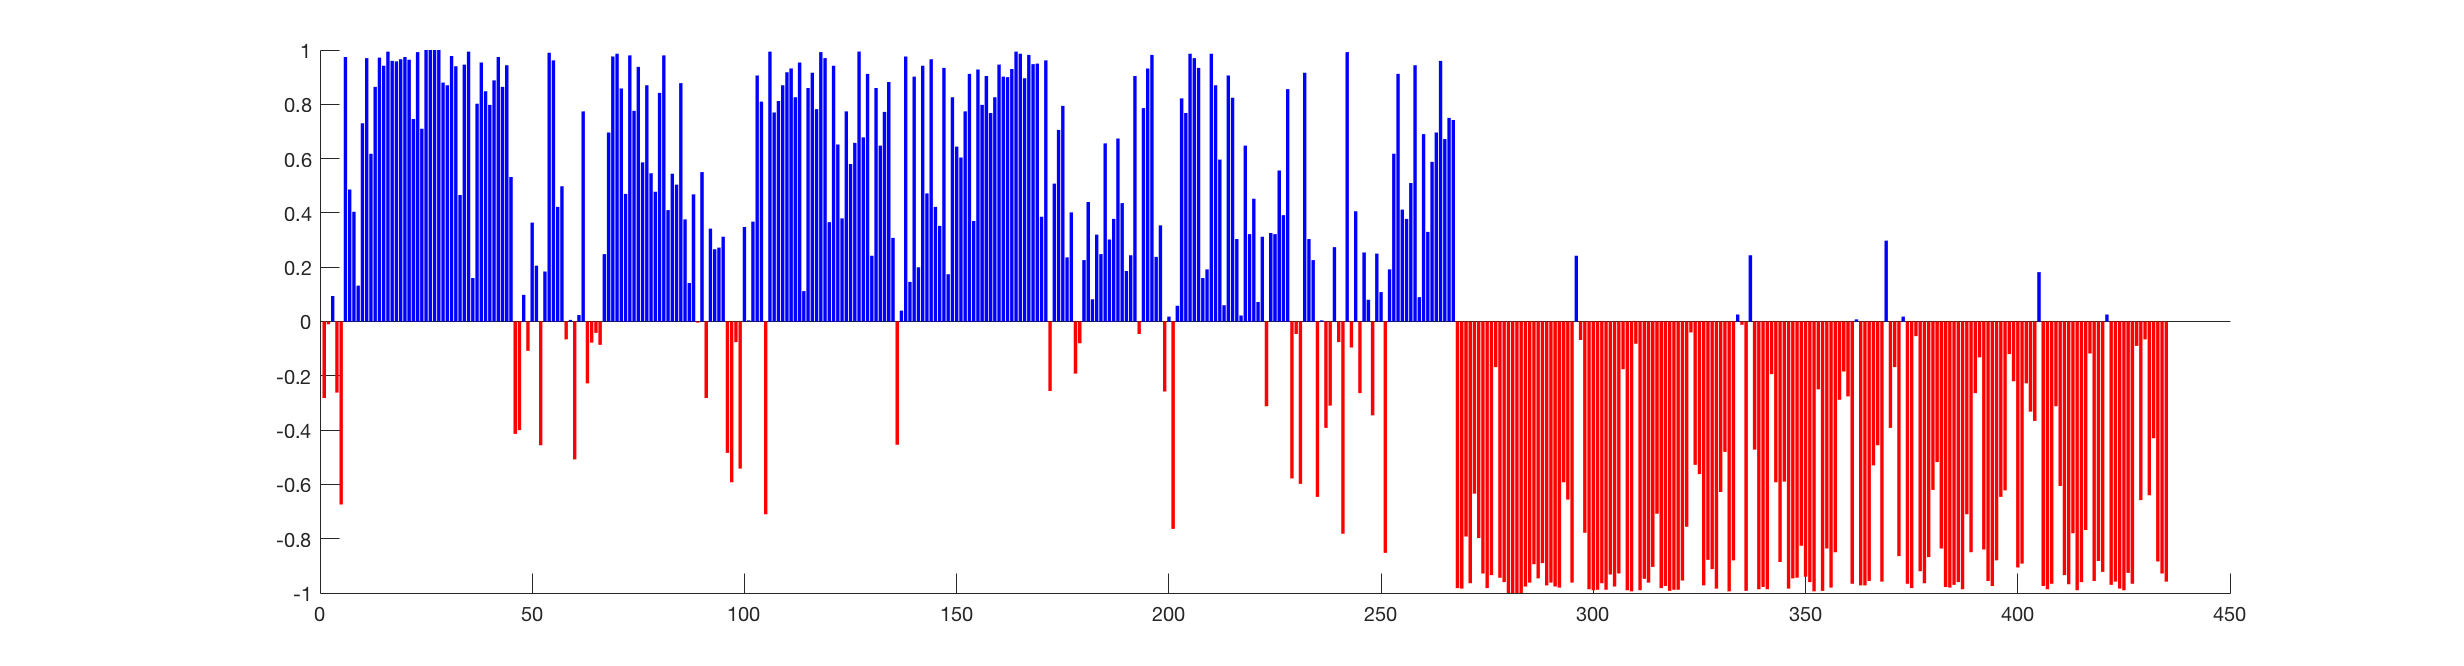
\includegraphics[width = \linewidth]{mcmc_gamma/manycorrect_clustering.png}
\end{figure}

I ran experiments with \cref{alg:hierarchical_tau_alpha} on the voting records data but plotting the traces of $\tau, \alpha$ and looking at the final average suggested that the Markov chain was not converging. We decided that the problem was in part due to the irregularity of the larger eigenvectors, perhaps because of the accuracy of Matlab's eig solver. Truncating the list of eigenvectors to only consider the first 50 seemed to help the problem, and we were able to observe better clustering. See \cref{fig:centered_voting_avg}, \cref{fig:centered_voting_tau}.

\begin{figure}[H]
\begin{minipage}{0.48\textwidth}
    \caption{\label{fig:centered_voting_avg} \cref{alg:hierarchical_tau_alpha} final average after truncating eigenvectors}
    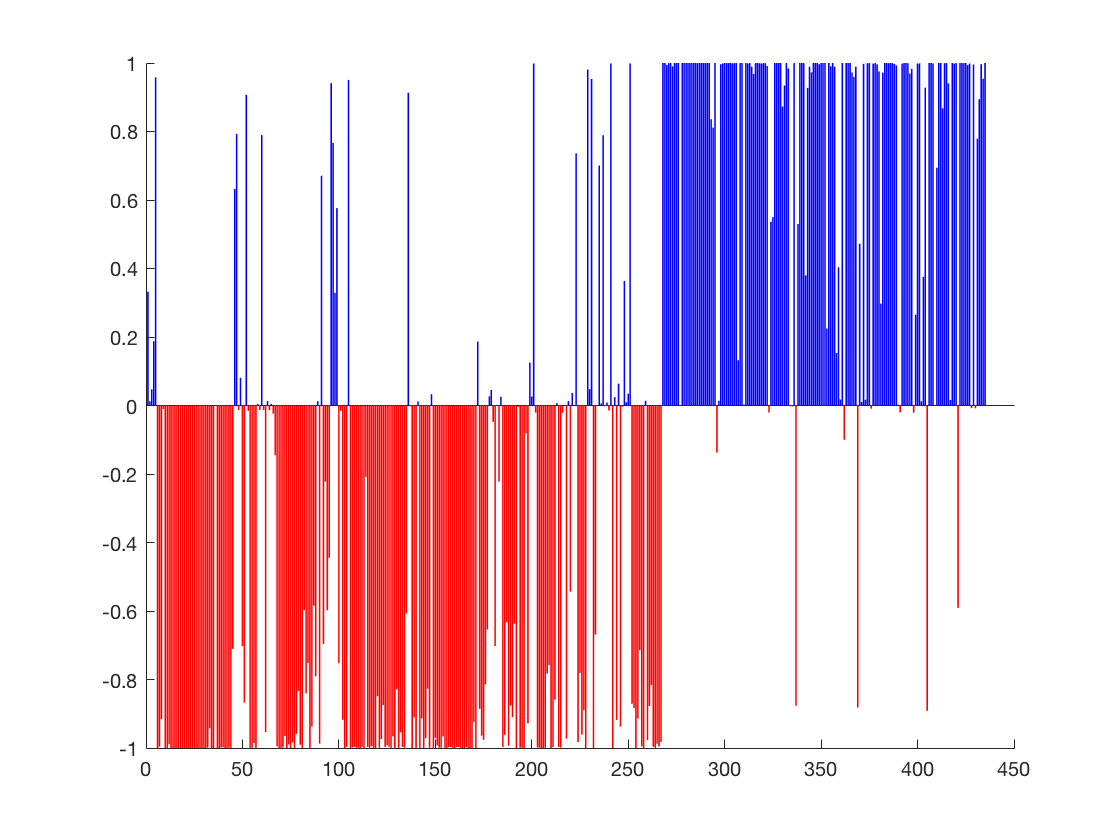
\includegraphics[width=\linewidth]{centered/final_avg.png}
\end{minipage}\hfill
\begin{minipage}{0.48\textwidth}
    \caption{\label{fig:centered_voting_tau} Trace of $\tau$}
    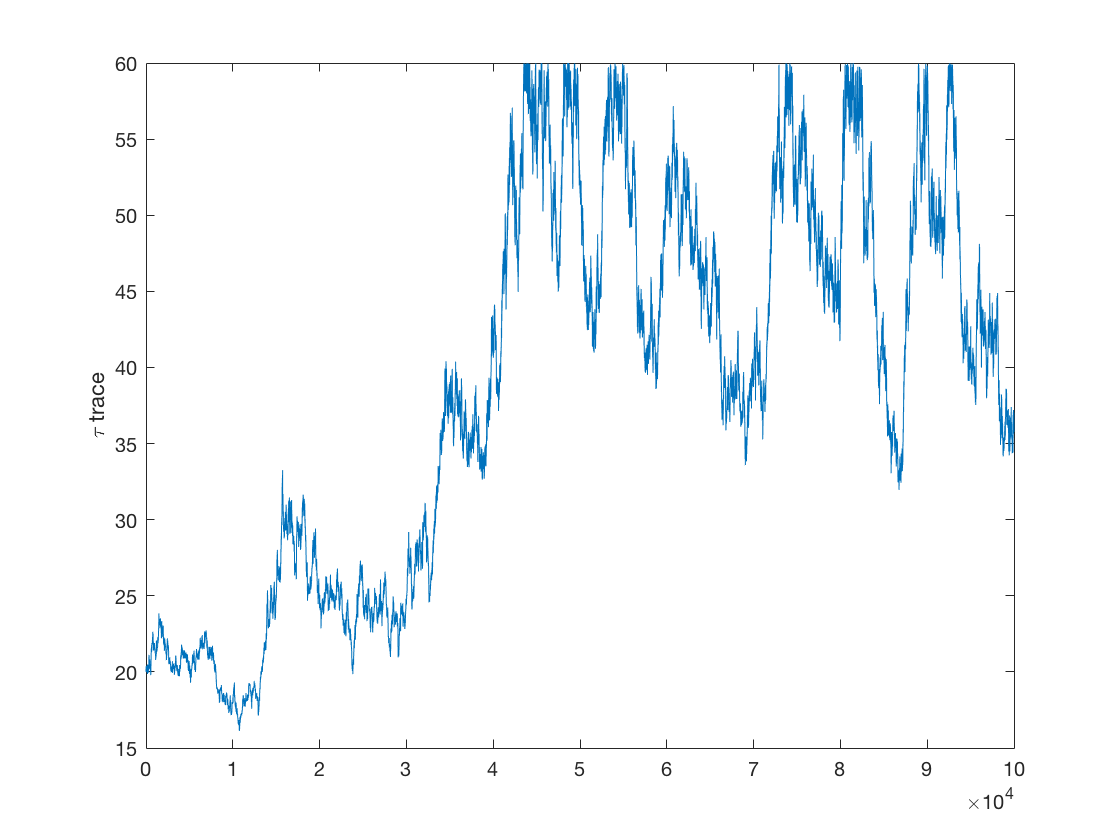
\includegraphics[width=\linewidth]{centered/trace_tau.png}
\end{minipage}
\end{figure}

Then, we compared the centered and non-centered algorithms. The non-centered \cref{alg:xi_tau_alpha} seems to converge faster than \cref{alg:hierarchical_tau_alpha}, and truncation of the eigenvectors is not necessary. See \cref{fig:noncentered_voting_avg}, \cref{fig:noncentered_voting_tau}

\begin{figure}[H]
\begin{minipage}{0.48\textwidth}
    \caption{\label{fig:noncentered_voting_avg}\cref{alg:xi_tau_alpha} final average}
    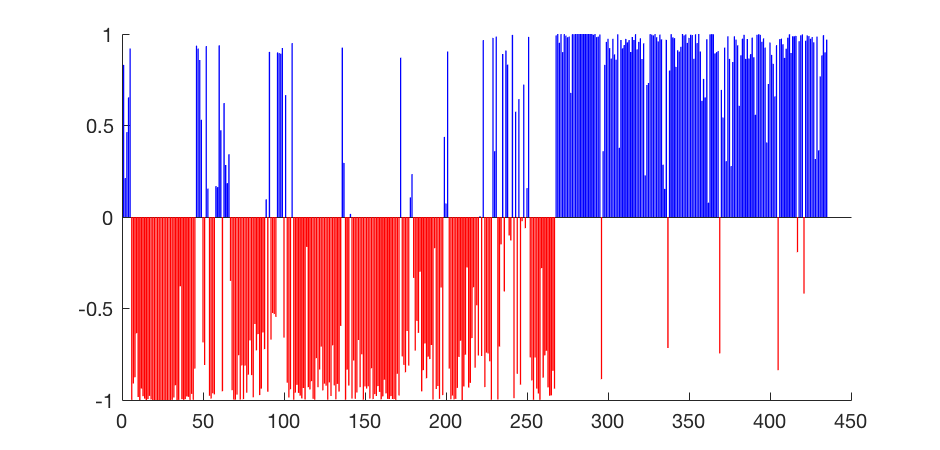
\includegraphics[width=\linewidth]{noncentered/final_avg.png}
\end{minipage}\hfill
\begin{minipage}{0.48\textwidth}
    \caption{\label{fig:noncentered_voting_tau} Trace of $\tau$}
    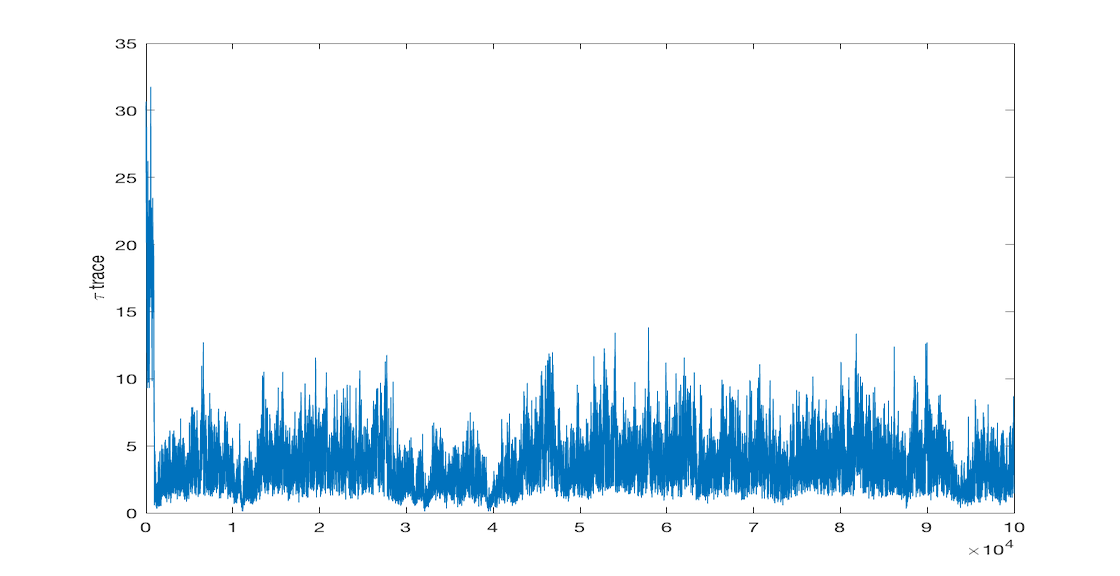
\includegraphics[width=\linewidth]{noncentered/trace_tau.png}
\end{minipage}
\end{figure}

Using these algorithms, I also ran experiments to cluster the two-moons data set. We explored using the self-tuning Laplacian, which was introduced in \cite{SelfTuning}. This Laplacian matrix has weights that infer the local spatial scale from the data, removing the need to choose a fixed length-scale parameter. The use of this self-tuning Laplacian in the two-moons data set seems to encode more information in the eigenvectors. Compare \cref{fig:moon_laplacian_un} with \cref{fig:moon_laplacian_selftuning}. 

\begin{figure}[!htb]
    \begin{minipage}{0.48\textwidth}
        \centering
        \caption{\label{fig:moon_laplacian_un} First eigenvectors of unnormalized Laplacian for intertwined moons data}
        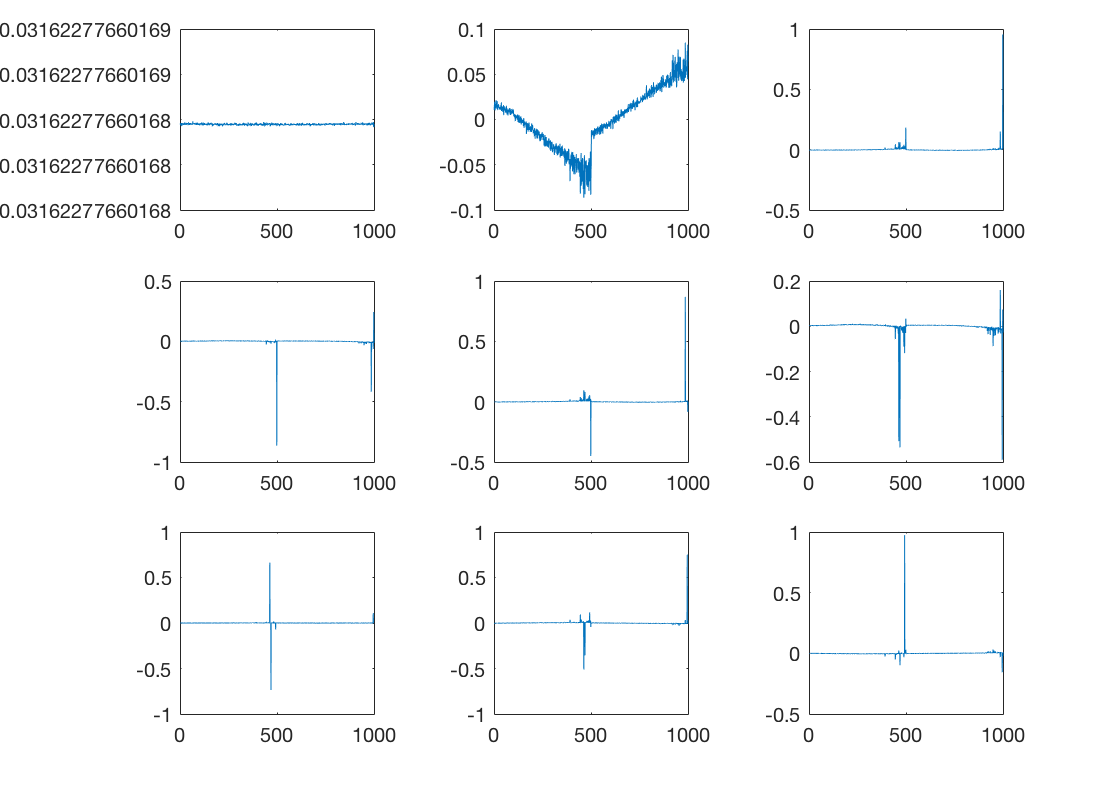
\includegraphics[width=\linewidth]{graphics/moon_laplacian_un.png}
    \end{minipage} \hfill
    \begin{minipage}{0.48\textwidth}
        \centering
        \caption{\label{fig:moon_laplacian_selftuning} First eigenvectors of unnormalized self-tuning Laplacian for intertwined moons data}
        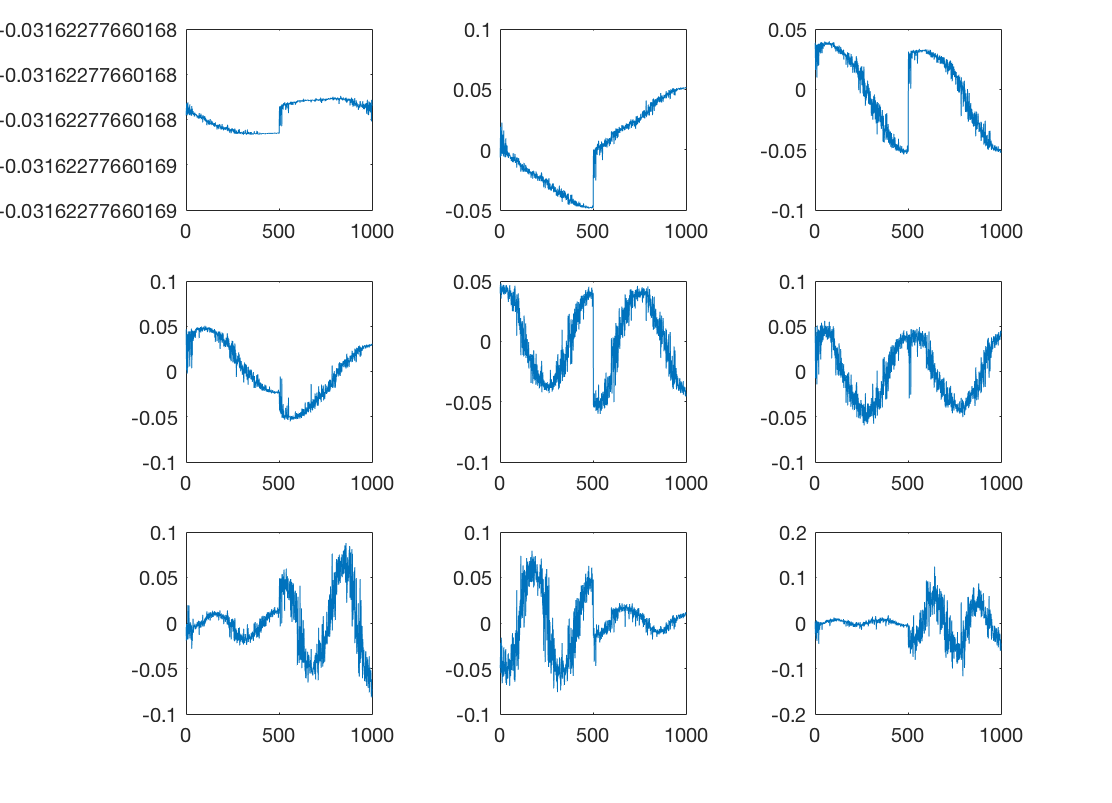
\includegraphics[width=\linewidth]{graphics/moon_laplacian_selftuning.png}
    \end{minipage}
\end{figure}

Compare the results from the centered, truncated algorithm and the non-centered self-tuning algorithm in \cref{fig:moon_centered_avg}, \cref{fig:moon_noncentered_avg}, \cref{fig:moon_centered_trace_tau}, \cref{fig:moon_noncentered_trace_tau}, \cref{fig:moon_centered_trace_alpha}, \cref{fig:moon_noncentered_trace_alpha}.
\begin{figure}[H]
    \begin{minipage}{0.48\textwidth}
        \centering
        \caption{\label{fig:moon_centered_avg} \cref{alg:hierarchical_tau_alpha} with truncation, final average}
        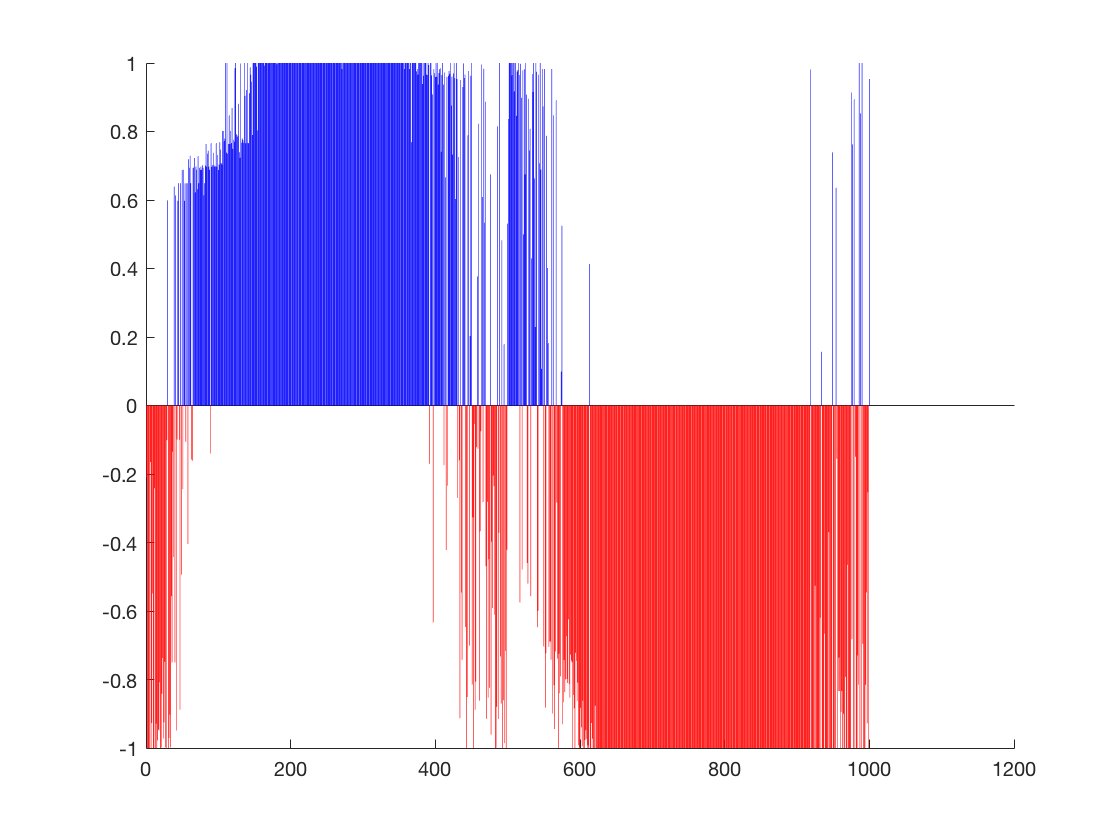
\includegraphics[width=\linewidth]{graphics/moons/centered_truncated/final_avg.png}
    \end{minipage} \hfill
    \begin{minipage}{0.48\textwidth}
        \centering
        \caption{\label{fig:moon_noncentered_avg} \cref{alg:xi_tau_alpha}, final average}
        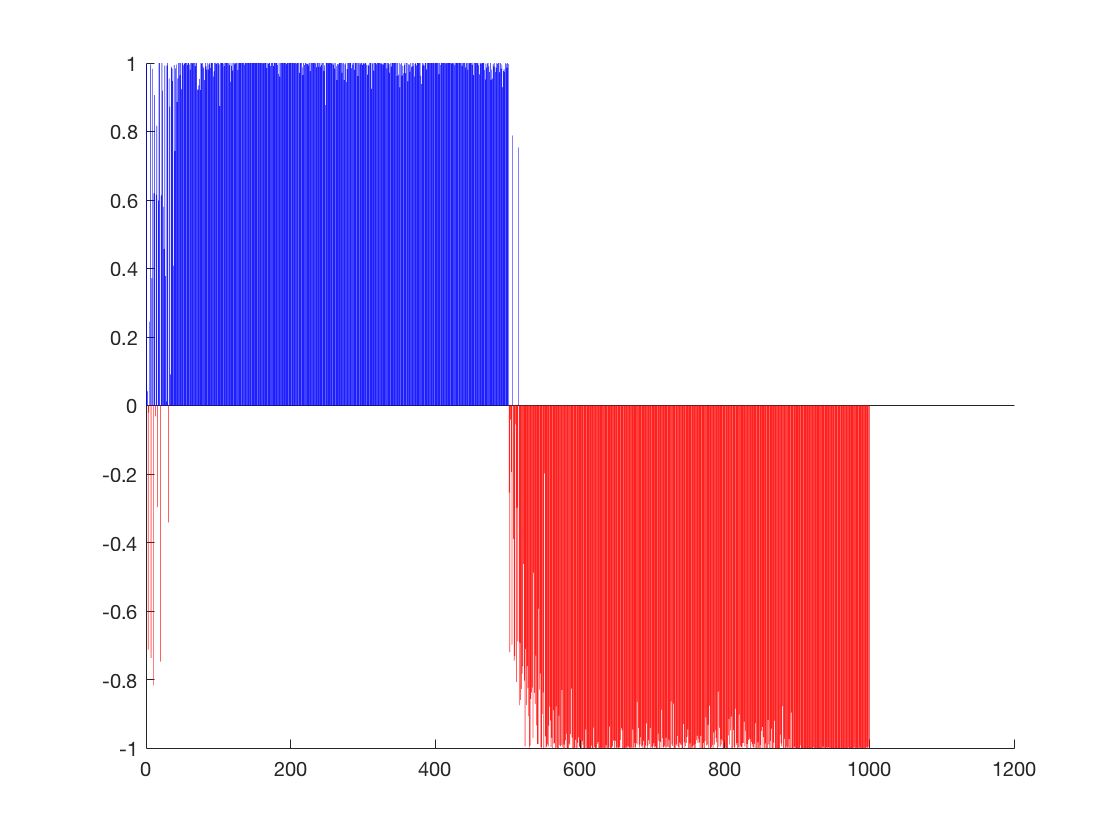
\includegraphics[width=\linewidth]{graphics/moons/noncentered_selftuning/final_avg.png}
    \end{minipage}
\end{figure}

\begin{figure}[H]
    \begin{minipage}{0.48\textwidth}
        \centering
        \caption{\label{fig:moon_centered_trace_tau} \cref{alg:hierarchical_tau_alpha} with truncation, trace $\tau$}
        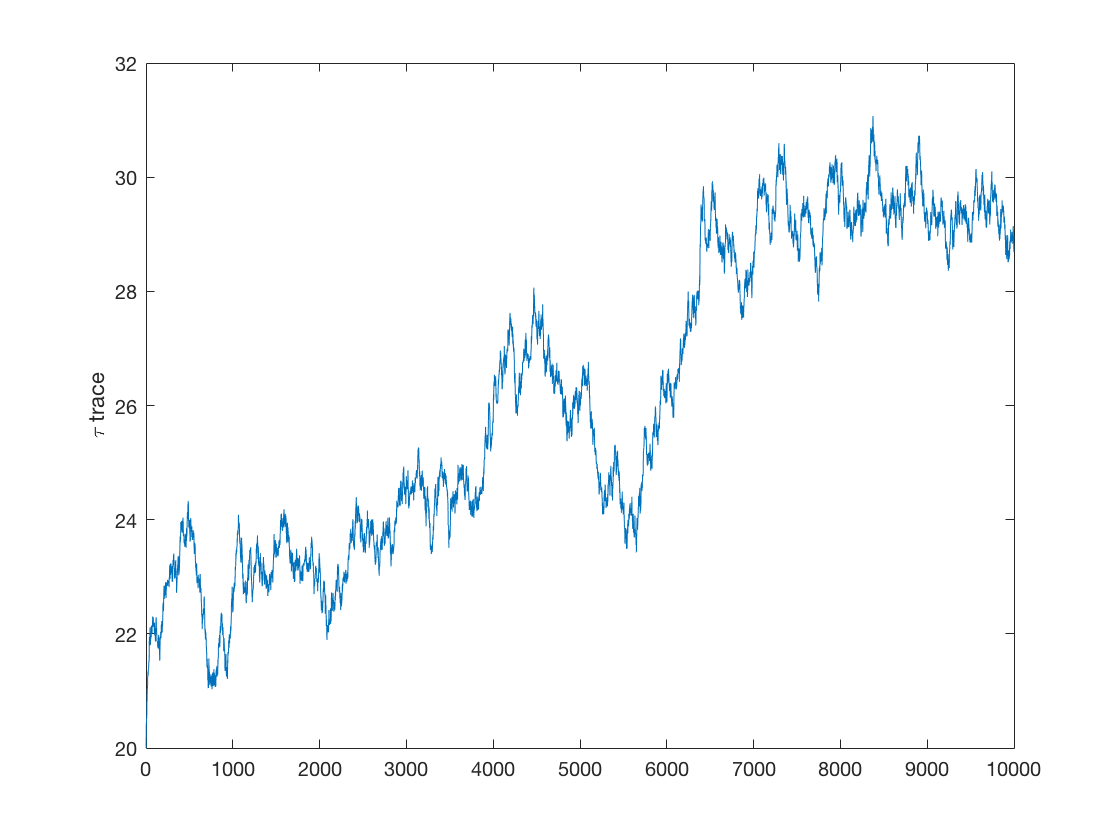
\includegraphics[width=\linewidth]{graphics/moons/centered_truncated/trace_tau.png}
    \end{minipage} \hfill
    \begin{minipage}{0.48\textwidth}
        \centering
        \caption{\label{fig:moon_noncentered_trace_tau} \cref{alg:xi_tau_alpha}, trace $\tau$}
        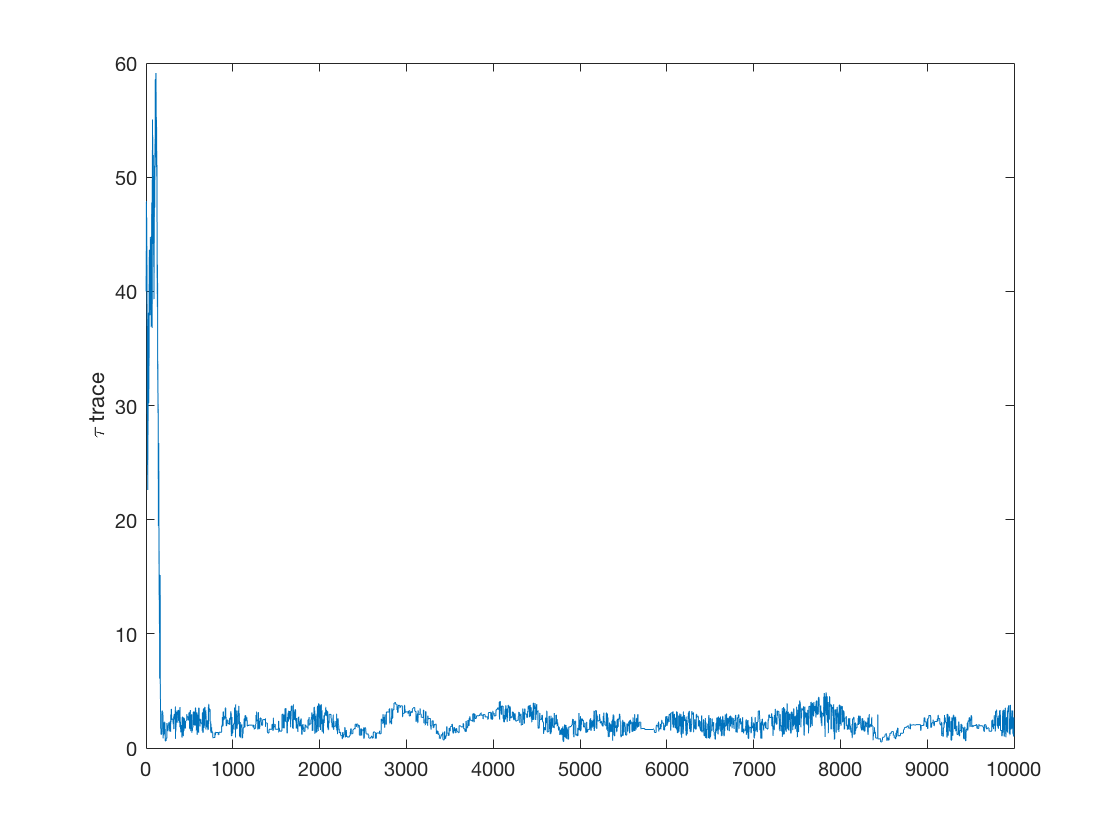
\includegraphics[width=\linewidth]{graphics/moons/noncentered_selftuning/trace_tau.png}
    \end{minipage}
\end{figure}

\begin{figure}[H]
    \begin{minipage}{0.48\textwidth}
        \centering
        \caption{\label{fig:moon_centered_trace_alpha} \cref{alg:hierarchical_tau_alpha} with truncation, trace $\alpha$}
        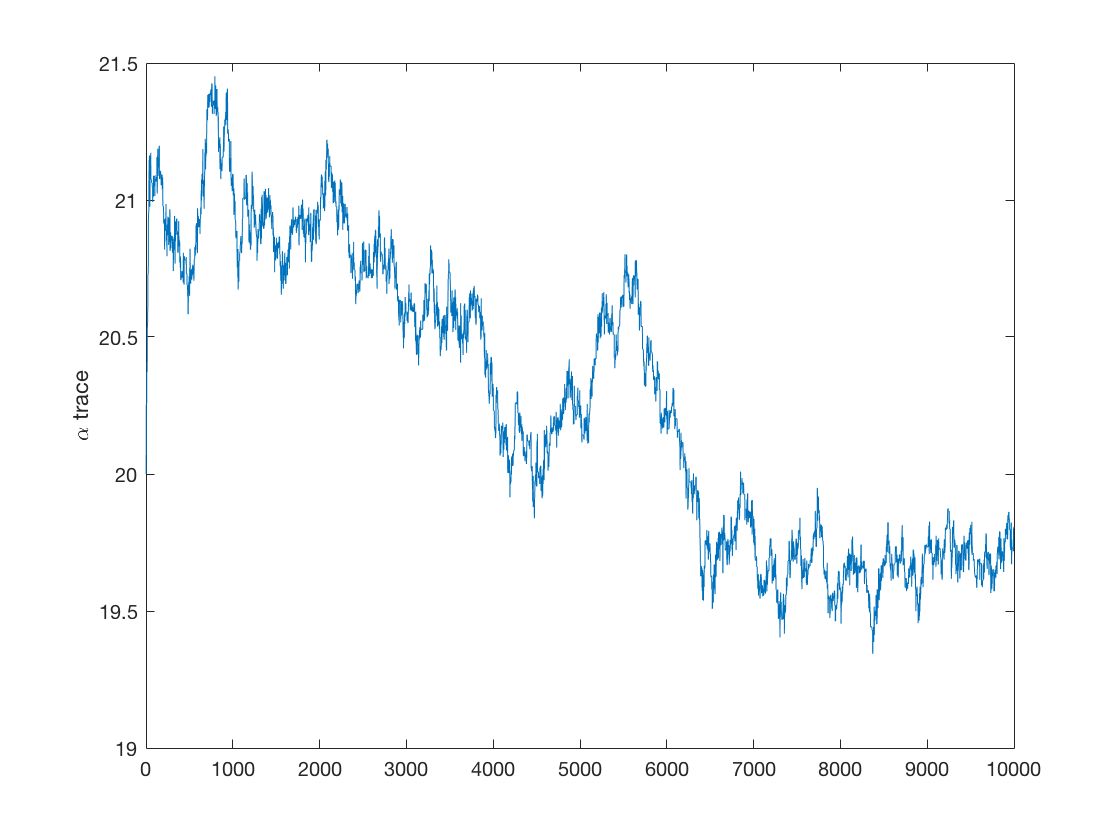
\includegraphics[width=\linewidth]{graphics/moons/centered_truncated/trace_alpha.png}
    \end{minipage} \hfill
    \begin{minipage}{0.48\textwidth}
        \centering
        \caption{\label{fig:moon_noncentered_trace_alpha} \cref{alg:xi_tau_alpha}, trace $\alpha$}
        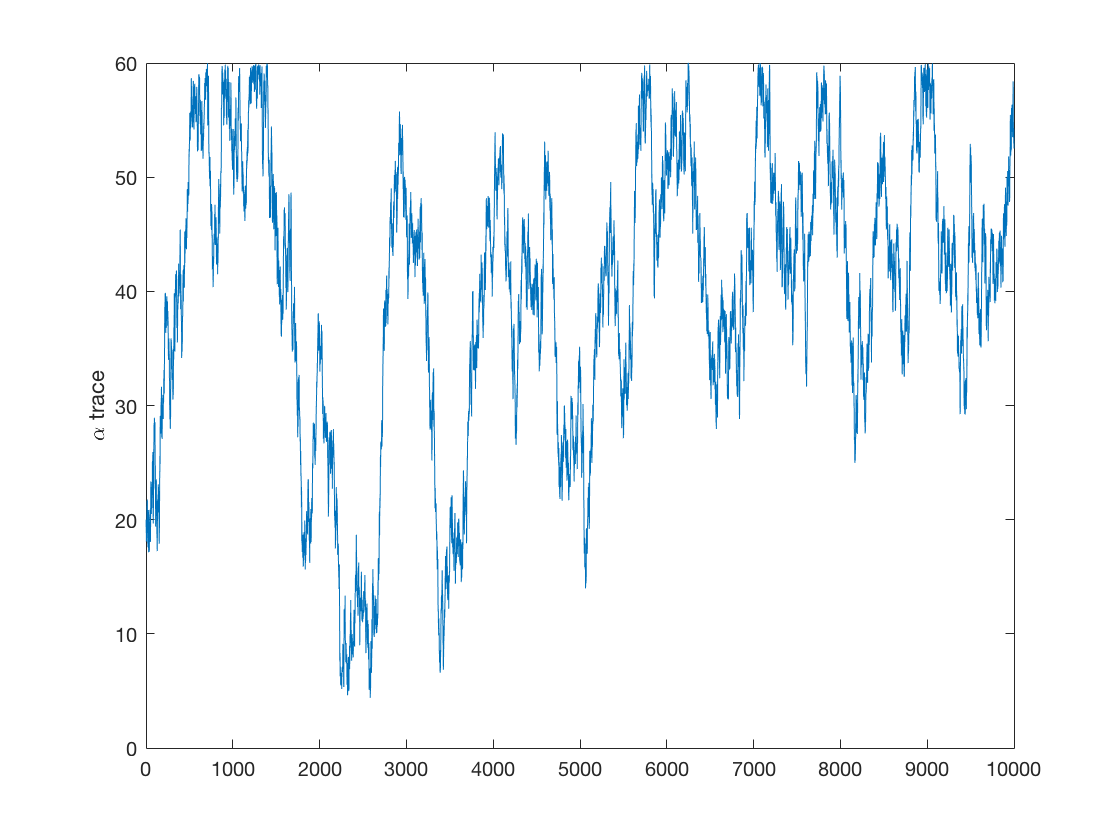
\includegraphics[width=\linewidth]{graphics/moons/noncentered_selftuning/trace_alpha.png}
    \end{minipage}
\end{figure}

Notice the convergence of $\tau$ and its low variance in the samples for the non-centered self-tuning algorithm. The distribution of $\tau$ is different between the two algorithms because truncating the number of eigenvectors affects the distribution of the posterior.

\section{Challenges}
Some common issues that I encountered are bugs in my Matlab code. Some of these bugs included overflow or underflow of ratios, when both numerator and denominator are very large or very small. To improve accuracy, I implemented these ratios as the difference between $\log$s, and took the $\exp$ of the result at the end. I became used to using Matlab's debugger to step through line-by-line and isolate the mistakes.

Another challenge was trying to get \cref{alg:hierarchical_tau_alpha}, the centered hierarchical algorithm, to perform well. The first implementation of that algorithm gave traces of the hyperparameters with low mixing and poor clustering of the voting records. Allowing for large ranges for $\tau$ and $\alpha$ did not solve the problem as the MCMC seemed to find one value of $\tau$ and stay stuck at that value. To try to debug the code, I re-implemented the algorithm using more of the linear algebra functionality of Matlab and improved the readability. This did not solve the problem, and we decided that the problem might have to do with the eig solver of Matlab failing for larger eigenvalues. We tested this by truncating the list of eigenvectors from $435$ down to only $50$, and the results, as mentioned above, were better. Since this fix is specific to these data sets, moving forward I anticipate that there may be more challenges with this algorithm. Note that the next step in the hierarchical models is to be hierarchical about this truncation level, which would tackle this problem.

We have also found that $\tau$ seems to have much lower variance than $\alpha$, and it is difficult to see if $\alpha$ has converged. To understand this problem, I have tried looking at histograms for $\alpha$ and saw that the distribution appears different from the prior distribution, since there seems to be a bias towards larger $\alpha$ (an example of this is in \cref{fig:moon_noncentered_trace_alpha}). We do not necessarily expect $\alpha$ to converge to a particular value -- it could just be that $\alpha$ is not strongly informed by the data. We have also observed high levels of correlation between $\tau$ and $\alpha$.

\section{Additional resources}
My project is mostly done on my computer, my notebook, and a whiteboard. Most likely, I will not require additional resources other than references to papers and books to read to understand the algorithms.

\bibliographystyle{siamplain}
\bibliography{references}
\end{document}